\documentclass[tikz,border=15pt]{standalone}
\usepackage{amsmath, amssymb}
\usetikzlibrary{arrows.meta}

\begin{document}
	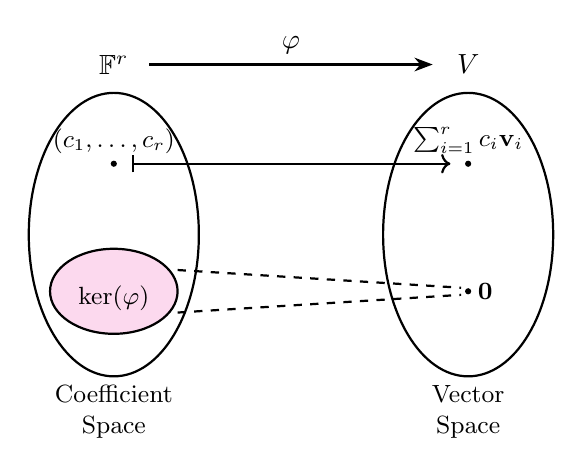
\begin{tikzpicture}[scale=.9]
		% Draw the domain and codomain sets
		\draw[thick] (-2,0) ellipse (1.2 and 2);
		\draw[thick] (3,0) ellipse (1.2 and 2);
		
		% Draw the Kernel subset inside the domain F^r
		\draw[thick, fill=magenta!15] (-2,-0.8) ellipse (0.9 and 0.6);
		\node[font=\small] at (-2, -0.9) {$\ker(\varphi)$};
		
		% Labels for the vector spaces (Top and Bottom)
		\node at (-2, 2.4) {$\mathbb{F}^r$};
		\node at (3, 2.4) {$V$};
		\node[font=\small, align=center] at (-2, -2.5) {Coefficient\\Space};
		\node[font=\small, align=center] at (3, -2.5) {Vector\\ Space};
		
		% Draw the arrow representing the linear map \varphi
		\draw[-Stealth, thick] (-1.5, 2.4) -- (2.5, 2.4) node[midway, above] {$\varphi$};
		
		% General element mapping
		\filldraw (-2, 1) circle (1pt) node[above, font=\small] {$(c_1,\dots,c_r)$};
		\filldraw (3, 1) circle (1pt) node[above, font=\small] {$\sum_{i=1}^{r}c_i\mathbf{v}_i$};
		\draw[|->, thick] (-1.75, 1) -- (2.75, 1);
		
		% Kernel mapping to the zero vector
		\filldraw (3, -0.8) circle (1pt) node[right, font=\small] {$\mathbf{0}$};
		
		% Dashed lines creating a "cone" to show the kernel crushing to zero
		\draw[dashed, thick] (-1.1, -0.5) -- (2.9, -0.75);
		\draw[dashed, thick] (-1.1, -1.1) -- (2.9, -0.85);
		
%		% Added explanatory labels pointing to specific parts
%		\draw[<-] (-2.9, -0.8) -- (-4, -0.8) node[left, font=\small, align=right] {All linear relations\\among $\mathbf{v}_1,\dots,\mathbf{v}_r$};
		
	\end{tikzpicture}
\end{document}